\chapter*{Management Summary}
\section*{Ausgangslage}

Mit dem \textit{cnlab TourLive System}, werden an Radrennsportanlässen Live- Informationen (Positions-, Bild- und Videodaten) gesammelt, verarbeitet und auf einer Webseite präsentiert. Das gegenwärtig eingesetzte System aus dem Jahr 2001  umfasst Nokia Symbian Aufnahmegeräte sowie einen PHP Webservice. TourLive wird an den verschiedensten Radrennsportanlässen in der Schweiz, unter anderem an der Tour de Suisse, eingesetzt. 
\\

In Zukunft soll \textit{TourLive} auch für kleinere Radrennsportanlässe zur Verfügung gestellt werden können. Dazu wurde im Rahmen dieser Bachelorarbeit das \textit{TourLive} System erneuert und erweitert. Neben den bestehenden Funktionalitäten soll im \textit{TourLive Next Generation}, kurs \textit{TourLive NG} der Fokus auf die Fernverwaltung der Aufnahmegeräte gelegt werden. 
\\

Als Partner und Auftraggeber dieses Projektes tritt die cnlab Software AG auf, die das bestehende System in Zusammenarbeit mit dem Radsportverband Swisscycling betreibt.

\section*{Vorgehen}
Nach eingehender Analyse des bestehenden Systems wurden in Zusammenarbeit mit der cnlab Software AG die Anforderungen an \textit{TourLive NG} spezifiziert. Als Basis diente die vorangegangene Analyse sowie die  Erfahrungswerte der cnlab Software AG aus den vergangenen Einsätzen. Mit Prototypen wurden einzelne Funktionen auf ihre Machbarkeit überprüft. Durch regelmässige Sitzungen mit der cnlab Software AG konnte fortlaufend auf Änderungswünsche eingegangen werden. Als Projektvorgehensmodell wurde in groben Zügen der Rational Unified Process \footnote{IBM RUP, \url{http://www-01.ibm.com/software/rational/rup/}, besucht am 25.04.2013} angewendet.
\newpage 

\section*{Ergebnisse}
Das neu entwickelte System \textit{TourLive Next Generation} basiert auf drei Komponenten wie folgende Abbildung zeigt. 
\begin{figure}[H]
	\centering
	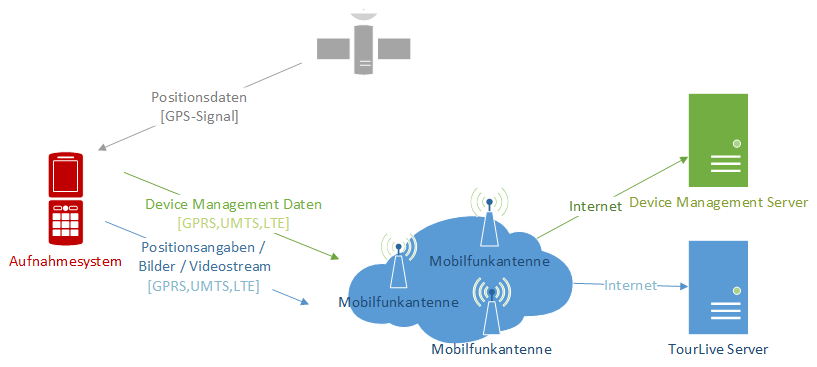
\includegraphics[width=140mm]{images/android/BigPicture_AndroidClient.png} 
	\caption{BigPicture TourLiveNG}
\end{figure}
Dies sind das auf Android basierende Aufnahmesystem, der TourLive Server und der Device Management Server. Der Geräteverwaltungsserver ermöglicht die Überwachung und Fernverwaltung der Aufnahmesysteme. Bei allfälligen Problemen ermöglicht ein Notfallwiederherstellungsdienst ein Neustart des Aufnahmesystems. Beide Serverkomponenten wurden mit dem Java Spring Framework realisiert. Sie verwenden zudem Twitter Bootstrap als GUI Framework und erfüllen damit unter Anwendung von \textit{\gls{rwd}} die Anforderung einer dynamischen Webseite die auch auf Tablets und Smartphones korrekt angezeigt wird. 
\\

Rennen und Etappen können komfortabel über die Passwort gesicherte Administrationsoberfläche des TourLive Servers verwaltet werden. Das Aufnahmesystem und die beiden Serverkomponenten kommunizieren über das \textit{\gls{http}} miteinander. Textdaten werden in einer JSON-Struktur übertragen während Video- und Bilddaten binär an den Server gesendet  werden. Der Videostream wird mit 10 sekündigen Videosequenzen realisiert die vom TourLive Server in ein vom Browser kompatibles Format konvertiert und mit Hilfes des HTML5 <video> Tags ausgeliefert werden. Aufgrund fehlender Standards und Browserinkompatibilitäten werden die Videosequenzen in verschiedenen Videoformaten zur Verfügung gestellt.


\section*{Ausblick}
\textit{TourLive NG} wurde in der Schlussphase des Projektes unter anderem an den Radsporttagen in Gippingen und an der zweiten Etappe der Tour de Suisse ausgiebig getestet. Die Tests haben gezeigt, dass das System grundsätzlich eingesetzt werden kann. Es wurden aber auch noch Optimierungsmöglichkeit eruiert und dokumentiert. Eine wichtige Erkenntnis dieser Testläufe ist die Problematik der Wärmeentwicklung der Geräte bei direkter Sonneneinstrahlung.
\\

Die Weiterentwicklung des Projektes liegt in den Händen der cnlab Software AG. Der Einsatz an weiteren Radrennen wird die cnlab Software AG gemeinsam mit dem Radsportverband Swisscycling prüfen.

